\documentclass[11pt, a4paper]{article}
\usepackage[utf8x]{inputenc}
\usepackage[swedish, english]{babel}		% last is active
\usepackage{graphicx}
\usepackage{amsmath}					% to be able to \split eqs
\usepackage{amssymb}					% Real/Imaginary fonts
\usepackage{units}
\usepackage[tight, hang]{subfigure}
\usepackage{url}
\usepackage{tikz}						% for drawing
\usetikzlibrary{shapes, arrows, decorations.markings, decorations.pathmorphing, decorations.pathreplacing, calc}
\usepackage{fancyhdr}
\usepackage{float}						% H-positioned and custom floats
\usepackage{datetime}					% to fix date format
\usepackage[usenames,dvipsnames]{pstricks}
%\usepackage{epsfig}
%\usepackage{pst-grad} % For gradients
%\usepackage{pst-plot} % For axes
\usepackage{pgfplots}
% =================== some local stuff ================= %
\newcommand{\degree}{\ensuremath{^\circ}}
\newcommand{\todayswe}{\the\year-\twodigit\month-\twodigit\day}


\def\contacts{Torbjørn Ludvigsen, tolu0022@student.umu.se\\Olof Lenti, olle0004@student.umu.se\\
Yunus Gures, yunusgures@gmail.com}
\def\names{Torbjørn Ludvigsen, Olof Lenti, Yunus Gures}
\def\dept{Department of Physics}
\def\course{Non-invasive measurement techniques}
\def\lab{Optical measurements:\\Determination of the Damping of a Pendulum with Time of Flight}
\def\supervisors{Patrick Ehlers\\Isak Silander\\ Amir Khodabakhsh}
\date{\todayswe}
% custom commands
\newcommand\OpVec[1]{\boldsymbol{\hat{#1}}}		% bold with hat for operator vectors
%\newcommand\Sup[1]{\textsuperscript{\tiny{#1}}}		% 1st, 2nd.. and so on
\newenvironment{eqn}{\begin{equation*} \begin{split}}{\end{equation*} \end{split}}
% header

% document
\begin{document}
\pagestyle{fancy}
\begin{titlepage}
	\begin{center}
		\course\\
		\Large{\lab}\vspace{2mm}
		\hrule\vspace{2mm}
		\tiny{\contacts}\vspace{2mm}
		\hrule
	\end{center}
	\vspace{4mm}

	\begin{abstract}

		\noindent In this report, a model of damping forces on a pendulum is derived and to some extent confirmed.
		The aim of the experiment is to find the different velocity regions for a pendulum in which different frictional forces are dominant.
		To achieve this, the velocities of two different pendula at their lowest points are measured.
		Time of flight with two laser beams and two photodiodes is the measurement method used.
		The main result is that the dominant frictional force of the  low-velocity regions of the pendula are of polynomial degrees 1.36(4) and 1.96(4).
		In the high velocity regions, the polynomial degree increases to 2.60(3) and 2.63(7).
		The only physical difference between the pendula is that the one with the higher polynomial degree in its friction force velocity dependency has a bigger area.

	\end{abstract}
	\vfill
	\hrule\vspace{2mm}
	\centering
		\tiny{Supervisor: \supervisors}
	%\end{center}
\end{titlepage}

\pagestyle{plain}
\vspace{2cm}
\section{Introduction}
A mechanical system consisting only of a rigid body, with only one degree of 
freedom, rotation around a constant axis, from here on called a pendulum, is 
a system of great interest. Historically it has had a wide range of
applications in science, mathematics and in everyday life. Among the reasons for
its continued importance as an educational tool in physics is its short, general 
equations of
motion in the linearized, small amplitude case, and the ease and the great number 
of ways by which this case can be extended.

This experiment in particular will measure a physical pendulum's decreasing velocity
in order to find and analyze its damping forces. A time of flight instrumentation
is constructed and used to acquire the velocity data.

\section{Theory}
\subsection{Time of Flight}
Time of Flight (ToF) is a method that measures the time for an object to travel a distance.
One can find either the distance of an object, its velocity or the length of the distance traveled with this technique, depending on what is known in the particular setup.

To measure the velocity with two measurement points, one needs to know the distance between them and measure the time it took.
This measured time is then equal to the distance between the measurement points divided by the velocity of the object.

\subsection{The pendulum}
For a rigid body pendulum affected by no frictional forces, using Newtons second law and balancing the
forces gives us the following
equation of motion:
\begin{equation}
  \frac{d^2\theta}{dt^2} + \frac{mgl\sin{\theta}}{I_p} = 0,
  \label{eq_of_motion}
\end{equation}
where $I_p$ is the bodys moment of inertia around the pivot point, $\theta$ is the
angle between the line through the pivot and the body's center of mass and the
vertical line, $m$ is the mass, $g$ is the acceleration due to gravity and
$l$ is the distance from the pivot point to the center of mass. 
Observe that the second derivative term corresponds to centrifugal forces, and
that the other term corresponds to gravitational ones.



%By approximating $\sin{\theta} \approx \theta$, we
%get the simpler expression
%\begin{equation}
%  \theta = Ae^{r_1t} + Be^{r_2t},
%  \label{diff_solution}
%\end{equation}
%where $A$, $B$ are constant determined by initial conditions and $r_1$, $r_2$ are
%solutions to the second order polynomial created by substituting equation
%\ref{diff_solution} into \ref{eq_of_motion}.

\subsubsection{Introducing Friction}
A physical pendulum will usually experience some friction between solid
surfaces around its pivot point.
This force may sometimes be modelled as being proportional to velocity\cite[p. 30]{book},
and sometimes as independent of velocity \cite{friction}.


To put both of these dependencies into Equation \ref{eq_of_motion}, 
we introduce a term $F_l = -A \frac{d\theta}{dt} - \text{sgn}\left(\frac{d\theta}{dt}\right)C$. 

\begin{equation}
    \frac{d^2\theta}{dt^2} 
  - A \frac{d\theta}{dt}
  + \frac{mgl}{I_p}\sin{\theta} 
  - \text{sgn}(\frac{d\theta}{dt})C 
  = 0,
  \label{eq_of_motion_comp1}
\end{equation}
where $A$ and $C$ are positive constants.
If $C = 0$ this now describes the motions of what is 
called a damped harmonic oscillator\cite{osc}.

\subsubsection{Introducing Drag}
Air drag is the frictional force between the air and the pendulum. 
This force is highly dependent on velocity.
For low velocities we approximate the air to be small evenly distributed balls,
bouncing off the
pendulum as it travels through space. 
Increasing velocity by some factor will increase the number of bouncing balls by the same
factor, so this introduces a linear term into 
Equation \ref{eq_of_motion_comp1}, and can be accounted for by adjusting the constant
$A$.

For higher velocities, however, this model breaks down, and the air must be
modeled as a fluid. Drag forces in fluids are proportional to the velocity
squared\cite{drag}, which for us means inserting a force 
$F_D = -B\cdot \left(\frac{d\theta}{dt}\right)^2$, where $B$ is a positive constant,
into Equation \ref{eq_of_motion_comp1}, giving us the equation of motion

\begin{equation}
    \frac{d^2\theta}{dt^2} 
  - B \frac{d\theta}{dt}
  \left(\left( 1 -   f\left(\frac{d\theta}{dt}\right)   \right ) + \frac{B}{A}f\left(\frac{d\theta}{dt}\right) \frac{d\theta}{dt} \right)  
  + \frac{mgl}{I_p}\sin{\theta} 
  - \text{sgn}\left(\frac{d\theta}{dt}\right)C
  = 0,
  \label{eq_of_motion_comp2}
\end{equation}
where $f(\omega)$ is a Heaviside step function evaluating to 1 if the angular
velocity is higher than some critical value:
\begin{equation}
f(\omega) = \left\{
  \begin{array}{lr}
    1 & : \omega > \omega_{c}\\
    0 & : \omega < \omega_{c}
  \end{array}
\right.
\label{e:heaviside}
\end{equation}

\subsubsection{Simplifying}

We can get a lot of information by looking at Equation \ref{eq_of_motion_comp2}
at the lowest point, where we know that gravitational and centrifugal forces
cancel each other and don't have any component in the direction of motion.

The force in this point will be negative:
\begin{equation}
  F = - B \frac{d\theta}{dt}
  \left(\left(1 - f\left(\frac{d\theta}{dt} \right)\right) + \frac{B}{A}f\left(\frac{d\theta}{dt}\right) \frac{d\theta}{dt} \right)  
  - \text{sgn}\left(\frac{d\theta}{dt}\right)C
\label{e:drag_comp}
\end{equation} 

\subsubsection{Energy Approach}
The equation of energy concerning angular velocity of the pendulum is
\[
	E = \frac{(\frac{d\theta}{dt})^2\cdot I_p }{2}.
\]
As $\frac{d\theta}{dt} = const\cdot v$ and $I_p$ is constant we can use the equation
\[
	E = d\cdot v_m^2,
\]
where $d$ is a constant and $v_m$ is the maximum motion of the bottom part of the pendulum, when calculating energies. 
The energies are demonstrated in Figure \ref{f:pendulummotion}.
\begin{figure}[h]
	\centering
	\includegraphics[scale=0.5]{pendulummotion}
	\caption{The energies of the moving pendulum are demonstrated.}
	\label{f:pendulummotion}
\end{figure}

We model the force of drag as in Equation \ref{e:drag_comp}, but with other constants and implicit Heaviside functions, like
\[
	F_d = a + bv + cv^2.
\]
The work done during one half period is found as
\[
	W = 2\int_0^s{F_d ds},
\]
where $s$ is the distance traveled by the bottom part of the pendulum during one fourth of a period.
Since $ds = rd\theta$ we get the equation
\[
	W = 2r\int_0^{\theta_m}{F_d d\theta},
\]
where $\theta_m$ is the turning angle.
We know that this work is much smaller than the total energy of the system. This is used to make the approximation 
\[
	mrg(1-\cos{\theta}) + \frac{mv^2}{2} = \frac{mv_m^2}{2} = \text{const},
\]
where $r$ is the length of the pendulum, $g$ is the acceleration of gravity, and $v_m$ is the maximum velocity of the pendulum, as shown in Figure \ref{f:pendulummotion}.
We can use this to find a relation between $d\theta$ and $dv$ as:
\[
	d\theta = \frac{kvdv}{\sqrt{1-(v^2+d)^2}},
\]
where $k$ is a constant and $d = 2rg - v_{m}^{2}$.
This is found by expressing $\theta$ as a function of $v$ and implicitly taking the derivative.
Using this we get an integral by which we can approximate the work.
\[
	W = 2kr\int_{v_m}^0 F_d \frac{kvdv}{\sqrt{1-(v^2+d)^2}}
\]
The velocities are not very high during our experiments. Thus we can Taylor expand around 0.
This integral is solved using Taylor expansion around 0 and Wolfram Alpha which gives us the equation:
\[
	W = \frac{av_{m}^{2}}{2\sqrt{2rg-d^2}} + \frac{bv_{m}^{3}}{3\sqrt{1-d^2}} + \frac{v_{m}^{4} (ad-cd^2+c)}{5(1-d^2)^{3/2}} + \mathcal{O}(5).
\]
Using the definition of $d$, which is a function of $v_m$ and Wolfram Alpha to Taylor expand the expression around $v_m=0$ we get the final equation for the work of one half period:
\begin{equation}
	W = A(a)v + B(b)v^2 + C(c)v^3 +  \mathcal{O}(4),
	\label{e:W}
\end{equation}
where A, B and C are new constants, still with the Heaviside function implicit. By taking the natural logarithm of both sides and making a linear fit the dominant polynomial can be found as the slope. 




\section{Experimental Setup}
The experimental setup consists of one electric circuit described in section 
\ref{s:Electric circuit}, one optical setup described in \ref{s:Optical setup}, a multifunction data acquisition card (DAQ), and 
a PC with MATLAB and LabVIEW installed. 
The setup can be seen in Figure \ref{f:setup}. 

\begin{figure}[h]
	\centering
	\includegraphics[scale=0.8]{setup}
	\caption{The experimental setup. From right to left we see the laser, the beam splitter, a lens, the pendulum, the second lens, the mirror, and the white circuit board.}
	\label{f:setup}
\end{figure}

\subsection{Electric circuit}
\label{s:Electric circuit}
The first mission is to convert light to voltage. This is done by using photodiodes 
that converts light into current, which is then converted using a
current-to-voltage converter.
Photodiodes are made from semiconductor materials and are based on p-n junctions that can easily get some of its electrons knocked into the conduction band by incident photons. 
We use Silicon photodiodes in the experiment. 
The electric circuit can be seen in Figure \ref{f:circuit}.
\begin{figure}[h]
	\centering
	\includegraphics{circuit}
	\caption{The electric circuit of the setup. D1 and D2 are the photodiodes.}
	\label{f:circuit}
\end{figure}

We connect a 100k$\Omega$ resistor from input to output to create an inverting amplifier. 
We feed the operational amplifier with 15V and we use a 470µF capacitor to reduce 
noise. The voltage is digitalized by a DAQ card that we attach to output of the 
amplifier. LabVIEW is used to collect the data.

\subsection{Optical setup}
\label{s:Optical setup}
The optical setup can be seen in Figure \ref{f:opticalsetup} and Figure \ref{f:setup}. 
We use a Helium-Neon 
laser (JDSU 1101) with a wavelength of 632.8nm. Firstly we set the laser, beam 
splitter, lenses and mirror on the same height. We get two parallel beams with the 
beam splitter. 
Obstructing the laser beam for a shorter time will sharpen the measured voltage spike, and thereby increase resolution of the measurements. 
We therefore hang a wire from the bottom of our pendulum, and point the laser at it rather than the pendulum body. 
We use two +100 mm lenses to make the beams as narrow as possible at the line of pendulum motion, as seen in Figure \ref{f:opticalsetup}.

\begin{figure}[h]
	\centering
	\includegraphics[scale=0.4]{opticalsetup2}
	\caption{The optical setup seen from above. A mirror is also used to direct the 
  lasers onto the photodiodes. The figure is not correct according to scale.}
	\label{f:opticalsetup}
\end{figure}

\section{Procedure}
Two measurement series is made. 
One with the bare pendulum, and one with some added area (the green plastic part shown in Figure \ref{f:setup}).
Only the velocities at the bottom point are recorded, not the period time.
The circuit voltage is measured 50 k times per second, and the LabView program detects when it rises above a certain threshold value.
When two voltage spikes has been detected, the time between them is written to a data file.
This time is then proportional to the inverse of the velocity, since the distance between the laser beams are constant.
The measured velocities have to be divided by the distance between the lasers in order to get units of m/s, but this is not done explicitly.

\subsection{Error of the slope of a linear fitting}
To calculate the error of the slope of a linear fit we simply use MATLAB to 
calculate the following equation:
\begin{equation}
	s = \text{std}(f(x)-data(x)),
	\label{e:std}
\end{equation}
where $s$ is the standard deviation of the residuals, $x$ is the x-values of the region considered, 
$data$ is the data values of the region considered and $f$ is the linear fit.
This standard deviation will be a measure of how correct the linear approximation is, 
but also gives an approximation of the total error from the time of flight instrumentation.

\section{Results}
In Figure \ref{f:nopaper} and Figure \ref{f:paper}, we see the logarithm of work done by friction and drag on the pendulum versus the logarithm of velocity, for a bare pendulum and one
with added area respectively. In both plots it is clear that there are two regions with different $v$-dependencies. 

The slopes and the errors of the linear fits of the two different regions of the plot in Figure \ref{f:nopaper} are calculated to be
\[
	k_{low} = \frac{\Delta\ln(W_{low})}{\Delta\ln(v_{low})} = 1.36(4),
\]
\[
	k_{high} = \frac{\Delta\ln(W_{high})}{\Delta\ln(v_{high})} = 2.60(3).
\]
The values inside the parentheses are the standard deviation of the residuals, calculated using Equation \ref{e:std}.

\begin{figure}[h!]
	\centering
	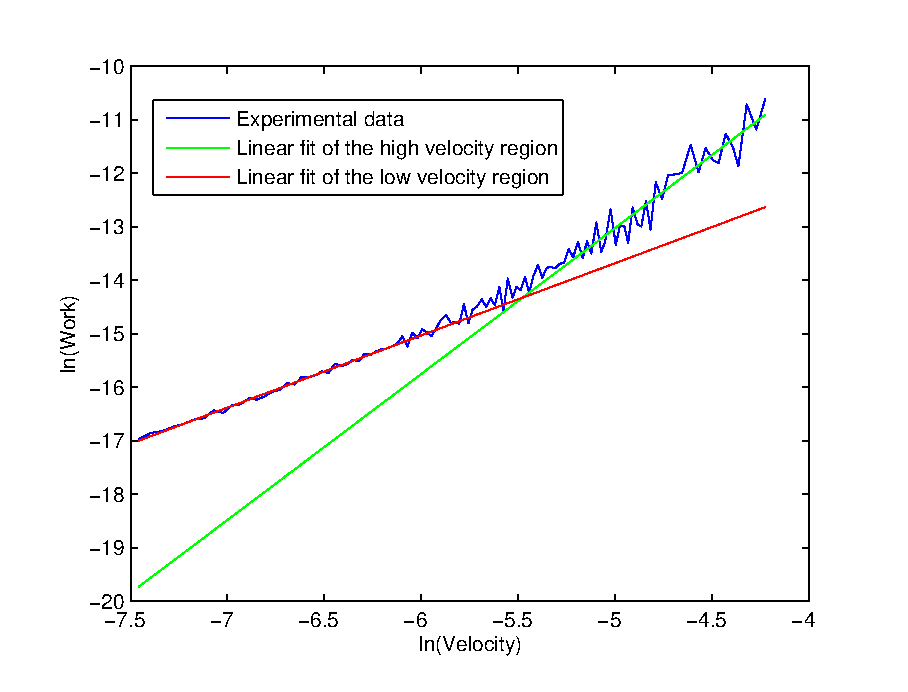
\includegraphics[trim=10.0cm 10.0cm 10.0cm 10.0cm, scale=0.7]{no_paper}
	\caption{Work versus velocity data and  linear fits for the bare pendulum.}
	\label{f:nopaper}
\end{figure}

In Figure \ref{f:paper} the slopes and the errors of the linear fits of the two different regions of the plot are calculated to be

\[
	k_{low}^{(A)} = \frac{\Delta\ln(W_{low})}{\Delta\ln(v_{low})} = 1.96(4),
\]\[
	k_{high}^{(A)} = \frac{\Delta\ln(W_{high})}{\Delta\ln(v_{high})} = 2.63(7).
\]

\begin{figure}[h!]
	\centering
	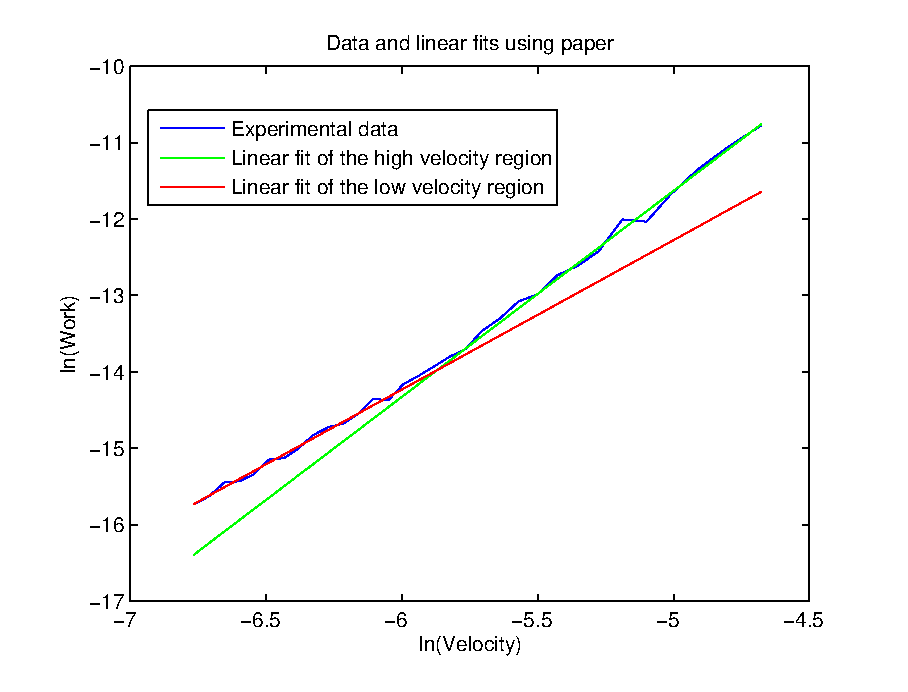
\includegraphics[trim=10.0cm 10.0cm 10.0cm 10.0cm, scale=0.7]{paper}
	\caption{Work versus velocity data and  linear fits for the pendulum with an added area.}
	\label{f:paper}
\end{figure}

It is clear that the slopes of the high velocity region are similar and close to $3$. 
The slope of the added-area pendulum for the low-velocity region is very close to $2$.
The slope of the bare pendulum for the low-velocity region is slightly above $1$.



\section{Discussion}
The experimentally retrieved plots values are very describing.
They verify the model described in Equation \ref{eq_of_motion_comp2} to some extent.
The critical velocity is clearly visible, and the slope in the low velocity region, especially for the added-area pendulum is very close to the expected value.

The behavior of the high-velocity region is not entirely as expected. 
We expected the slope of the added-area pendulum to be closer to $3$ than the slope in the high-velocity region of the other pendulum.
This is explained by the fact that the high-velocity regions are not exactly the same for the different types of pendula. 
We were not able to do a high enough velocity measurement due to the quick damping as well as the fluttering of the added area.

The fact that neither $k_{high}$ or $k_{high}^{(A)}$ are closer to 3 is explained by the velocities of the pendulum around its turning point.
In this area the pendulum will experience linear drag according to our model. 
 
 \section{Summary and Conclusions}
The friction on an object traveling through air, give rise to forces with a discontinuous dependency of velocity.
Between the discontinuous break-points there are continuous dominant polynomial dependencies arising from friction between solid surfaces, linear drag or quadratic drag.
In our plots we see three different regions of friction and drag, depending on the shape and velocity of the pendulum. 
Solving the general equation of pendulum motion is not needed to see this tendency.

There should be a more elegant way to get the equation of work than the one described in this report. 
We were not able to find this.

\vfill

\begin{thebibliography}{99}

  \bibitem{book} Baker, Blackburn (2005). 
  \textit{The Pendulum, A Case Study in Physics}\\
  Oxford, University Press.

  \bibitem{friction} Wikipedia. \textit{Friction}\\ 
  \url{http://en.wikipedia.org/wiki/Friction} [\todayswe]
	
  \bibitem{osc} Wikipedia. \textit{Harmonic oscillator}\\ 
  \url{http://en.wikipedia.org/wiki/Harmonic_oscillator} [\todayswe]

  \bibitem{drag} Wikipedia. \textit{Drag}\\ 
  \url{http://en.wikipedia.org/wiki/Drag_(physics)} [\todayswe]

\end{thebibliography}

\begin{appendix}
\end{appendix}

% nY KOMMENTAR

\end{document}
%\begin{figure}[H]
%	\centering
%	\begin{tikzpicture}[scale = 0.95]
%		\def\mr{1.5};
%		\draw (0,0) ellipse (0.5 and \mr);
%		\begin{scope}
%			\clip (0,0) ellipse (0.5 and \mr);
%			\foreach \i in {0, 1, ..., 15} {
%				\draw (-0.5, {-3 + 0.25*\i}) -- (0.5, {-1 + 0.25 * \i});
%			}
%		\end{scope}
%		\path[fill = white, opacity = 0.7] (0, 0) circle (0.2);
%		\node at (0, 0) {$S$};
%		\begin{scope}
%			% overlapping regions will cancel out
%			\draw[fill = white] (5, 0) circle (3);
%		\end{scope}
%		\draw (0, \mr) -- ++(2.8, 0) to[out = 0, in = -135] ++(0.3, 0.3)
%			  (0, -\mr) -- ++(2.8, 0) to[out = 0, in = 135] ++(0.3, -0.3);
%		\node at (5, 0) {$V$};
%	\end{tikzpicture}
%	\caption{Helmholtz resonator}
%	\label{f:helmholtz}
%\end{figure}
